\documentclass[addpoints, 12pt] {exam}
\usepackage{graphicx}
\usepackage{amsmath}
\bracketedpoints
\pagestyle{headandfoot}
\runningheadrule
\firstpageheader{Math 112}{Written Homework 4}{Due February 9th 2024}
\runningheader{Math 112}{ Page\; \thepage\; of\; \numpages}{Written Homework 4}
\firstpagefooter{}{}{}
\runningfooter{}{}{}
\setlength\answerskip{2ex}
\setlength\answerlinelength{1.5in}
\begin{document}

\begin{center}
\fbox{\fbox{\parbox{5.5in}{\centering
Directions:\\Please only put your final, well written solutions, in the space provided.\\ Give exact answers (simplified radicals or fractions).\\If you use additional paper clearly label the question and upload pages after the question page.\\Use complete sentences and explain your reason as much as possible.\\There are \numquestions\,  questions and \numpoints\, points total
}}}\end{center}
\vspace{0.1in}
\makebox[\textwidth]{Name:\enspace\hrulefill}
%\qformat{Question \thequestion \dotfill \thepoints}%

\begin{questions}
\question Jorge earns \(\$27.50\) per hour, up to \(40\) hours per week. 
\begin{parts}
\part[2] Write a function representing Jorge's income as a function of the hours they work during the week.
\vspace{0.25in}
\answerline
\part[1] What is the domain for this function?\answerline
\part[2] Jorge earns ``time-and-a-half'' for any time worked \emph{over} 40 hours. Write a function that represents their income if they work over 40 hours.\vspace{1in}\answerline
\part[1] What is the domain for this new function of their income?\answerline
\part[1] Rather than dealing with two separate calculations, create a single, piecewise function, that represents Jorge's income as a function of hours worked:\newpage
\part[3] Sketch the graph of the piecewise function. You may use a separate paper if you wish. \newpage
\end{parts}
\question To enroll in a phone plan, you shop around various vendors and find one you like. They offer the following data plan: The initial setup fee is $\$100$ and the first 5 gigabytes are priced at $\$2$ per gigabyte. Any additional data is priced at $\$10$ per gigabyte. 
\begin{parts}
\part[4] What is the piecewise function that represents the cost for $x$ gigabytes of data? \vspace{2in}
\part[4] Graph the function with an appropriate scale and indicate {\bf all important points} such as intercepts, intersections, and cutoff values for the piecewise function. Be sure to label your axes and indicate clearly the scale. \vspace{2in}
\part[2] How much will it cost you to use $12$ gigabytes of data?
\answerline
\end{parts}\newpage
\question When companies make bulk purchases, it is often possible to get a reduced cost per item. A particular wholesaler of novelty pens sells their pens for \(\$0.95\) per pen on order less than \(300\). For orders of more than \(300\) pens, the price drops to \(\$0.75\) per hat. 
\begin{parts}
\part[4] Express the total cost as a function of the number of pens purchased.\vspace{2in}\answerline
\part[4] Sketch the graph of this function. You may use a separate piece of paper.\vspace{4in}
\part[2] Suppose you are making a purchase on behalf of an organization that has raised \(\$300\).  What is the most amount of pens you could purchase?
\answerline\newpage
\end{parts}
\question Below is the graph of a piecewise function
\begin{center}
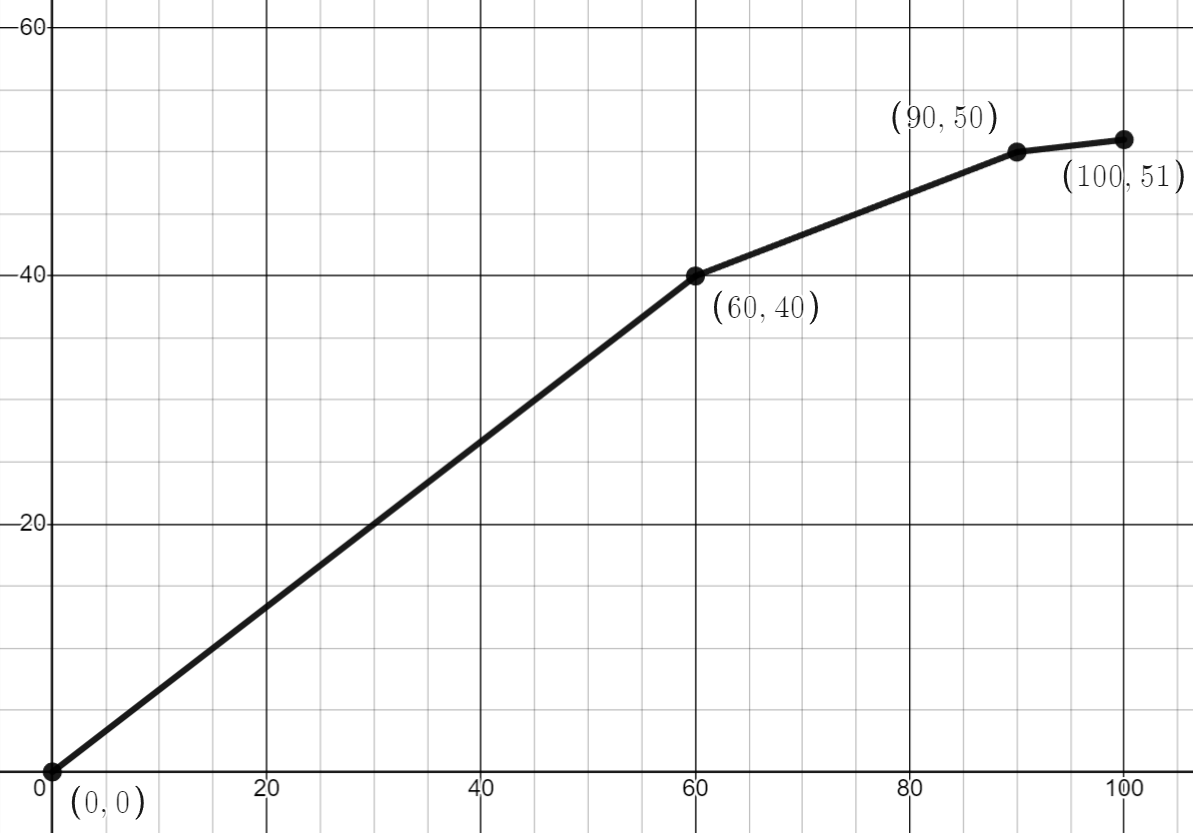
\includegraphics[scale=0.4]{piecewisehw4}
\end{center}
\begin{parts}
\part[1] What is the domain of this function?\answerline
\part[1] What is the range of this function?\answerline
\part[1] Where is the function increasing?\answerline
\part[1] Where is the function decreasing?\answerline
\part[6] Write a piecewise function definition for this graph. 
\end{parts}
\end{questions}


\end{document}